\newcommand{\microns}{$\upmu$m\xspace}
\newcommand{\etal}{\textit{et al.}\xspace}
\newcommand{\Ef}{$E_{F}$\xspace}
\newcommand{\SiO}{SiO$_{2}$\xspace}
\newcommand{\insitu}{\textit{in situ}\xspace}
\newcommand{\Ohms}{$\Omega$\xspace}


\newcommand{\InsertFig}[3]{
  \begin{figure}[!htbp]
    \begin{center}
      \leavevmode
      #1
      \caption{#2}
      \label{#3}
    \end{center}
  \end{figure}
}



\documentclass[oneside,11pt]{Classes/myThesis}
%%%%%%%%%%%%%%%%%%%%%%%%%%%%%%%%%%%%%%%%%%%%%%%%%%%%%%
%%%%%%%%%%%%%%%%%%% Instructions %%%%%%%%%%%%%%%%%%%%%
%%%%%%%%%%%%%%%%%%%%%%%%%%%%%%%%%%%%%%%%%%%%%%%%%%%%%%
%% Fill in the details about your name, and project title
%% in the sections just below here. Then you write each
%% Chapter in a separate LaTeX file - you will find Chapter 1
%% is already setup for you.
%%
%% The folder structure is:
%% Chapters
%%     |-----------> Chapter_1
%%     |                  |----------> Chapter_1_Fig
%%     |                  |               |-> My_fig.eps
%%     |                  |----------> Chapter_1_file.tex
%%     !-----------> Chapter_2
%%     |                  |----------> Chapter_2_Fig
%%     |                  |               |-> My_other_fig.eps
%%     |                  |----------> Chapter_2_file.tex
%%
%% Chapter_1 contains an exa,ple of includinga figure in the text with a reference.
%%%%%%%%%%%%%%%%%%%%%%%%%%%%%%%%%%%%%%%%%%%%%%%%%%%%%%
%%%%%%%%%%%%%%% file path for figures - add extra chapters as necessary %%%%%%%%%
%%%%%%%%%%%%%%%%%%%%%%%%%%%%%%%%%%%%%%%%%%%%%%%%%%%%%%
\graphicspath{{./Chapters/Chapter_1/Chapter_1_Fig/}     
              {./Chapters/Chapter_2/Chapter_2_Fig/}
              {./Chapters/Chapter_3/Chapter_3_Fig/}
              {./ThesisFigs/}}

%%%%%%%%%%%%%%%%%%%%%%%%%%%%%%%%%%%%%%%%%%%%%%%%%%%%%%
%%%%%%%%%%%%% Constants - fill these in for use throughout the thesis %%%%%%%%%%%%
%%%%%%%%%%%%%%%%%%%%%%%%%%%%%%%%%%%%%%%%%%%%%%%%%%%%%%
\newcommand{\theAuthor}{Your Full name}
\newcommand{\authorEmail}{physpqr@leeds.ac.uk}
\newcommand{\myTitle}{My Project  Title}
\newcommand{\supervisor}{Prof. M.Y. Supervisor}
%%%%%%%%%%%%%%%%%%%%%%%%%%%%%%%%%%%%%%%%%%%%%%%%%%%%%%
\pdfinfo { /Title  (\myTitle)
           /Creator (TeX)
           /Producer (pdfTeX)
           /Author (\theAuthor \authorEmail)
           /ModDate (D:\pdfdate)
           /CreationDate (D:\pdfdate)  %format D:YYYYMMDDhhmmss
           /Subject (Condensed Matter Physics)
           /Keywords (BSc, Report)}    
		\pdfcatalog { /PageMode (/UseOutlines)
                  /OpenAction (fitbh)  }

%%%%%%%%%%%%%%%%%%%%%%%%%%%%%%%%%%%%%%%%%%%%%%%%%%%%%%
%%%%%%%%%%%%% Title Page Information %%%%%%%%%%%%%%%%%%%%%%%%%%%%
%%%%%%%%%%%%%%%%%%%%%%%%%%%%%%%%%%%%%%%%%%%%%%%%%%%%%%
\title{\myTitle}
\author{\href{mailto:\authorEmail}{\theAuthor}}
\crest{
\includegraphics[width=35mm]{Leeds_Crest.png}}
%%%%%%%%%%%%%%%%%%%%%%%%%%%%%%%%%%%%%%%%%%%%%%%%%%%%%%
%% Define these as empty to omit the two logos on the title page
%%%%%%%%%%%%%%%%%%%%%%%%%%%%%%%%%%%%%%%%%%%%%%%%%%%%%%
\logo{} %\includegraphics[width=50mm]{UoL_logo}} %University Logo
\deptlogo{} %\includegraphics[width=50mm]{UoL_logo}} % Institute Logo
%%%%%%%%%%%%%%%%%%%%%%%%%%%%%%%%%%%%%%%%%%%%%%%%%%%%%%
\collegeordept{\href{http://physics.leeds.ac.uk}{School of Physics and Astronomy}}
\university{\href{http://www.leeds.ac.uk}{University of Leeds}}

\degree{Bachelor of Science}
\degreedate{\monthdate\today}

%Different font in captions
%Different font in caption
%%%%%%%%%%%%%%%%%%%%%%%%%%%%%%%%%%%%%%%%%%%%%%%%%%%%%%
%%%%%%%%%%%%%%%% Optional Packages  %%%%%%%%%%%%%%%%%%%%%%%%%%%
%%%%%%%%%%%%%%%%%%%%%%%%%%%%%%%%%%%%%%%%%%%%%%%%%%%%%%
%\usepackage{StyleFiles/watermark}
%\usepackage{xspace}  %add a space after maths if not already there
%\usepackage{booktabs} %better tables
%\usepackage{rotating}  %rotating figures and tables
% \usepackage{array} %enhanced tables
%\usepackage{ctable} %include a figure command
%\usepackage{footnote}
%\usepackage{multirow} %for merging cells on tables
%\usepackage{times} % The "Times" font
%\usepackage{Utopia} % The "Utopia" font

\linespread{1.3} %1.5 line spacing

\begin{document}
%\baselineskip=18pt plus1pt

\maketitle
%set the number of sectioning levels that get number and appear in the contents
\setcounter{secnumdepth}{2}
\setcounter{tocdepth}{2}
\pagenumbering{roman}
\frontmatter
%%%%%%%%%%%%%%%%%%%%%%%%%%%%%%%%%%%%%%%%%%%%%%%%%%%%%%
%%%%%%%%%%%% Include sections are required, or comment out to skip over %%%%%%%%%
%%%%%%%%%%%%%%%%%%%%%%%%%%%%%%%%%%%%%%%%%%%%%%%%%%%%%%
%% Thesis Dedictation ---------------------------------------------------

\begin{dedication} %this creates the heading for the dedication page

To my Mum, without her help these past 27 years there's no way I would have gotten this far.

Thank you so much, for everything.

\end{dedication}

% ----------------------------------------------------------------------

%%% Local Variables: 
%%% mode: latex
%%% TeX-master: "../thesis"
%%% End: 

% Thesis IP Statement ---------------------------------------------------

\begin{ipstatement} %this creates the heading for the dedication page

I am aware that the University defines plagiarism as presenting someone else’s work, in whole or in part, as your own. Work means any intellectual output, and typically includes text, data, images, sound or performance.

I promise that in the attached submission I have not presented anyone else’s work, in whole or in part, as my own and I have not colluded with others in the preparation of this work. Where I have taken advantage of the work of others, I have given full acknowledgement.I have not resubmitted my own work or part thereof without specific written permission to do so from the University staff concerned when any of this work has been or is being submitted for marks or credits even if in a different module or for a different qualification or completed prior to entry to the University. I have read and understood the University’s published rules on plagiarism and also any more detailed rules specified at School or module level.I know that if I commit plagiarism I can be expelled from the University and that it is my responsibility to be aware of the University’s regulations on plagiarism and their importance.

I re-confirm my consent to the University copying and distributing any or all of my work in any form and using third parties (who may be based outside the EU/EEA) to monitor breaches of regulations, to verify whether my work contains plagiarised material, and for quality assurance purposes. 

I confirm that I have declared all mitigating circumstances that may be relevant to the assessment of this piece of work and that I wish to have taken into account.I am aware of the University’s policy on mitigation and the School’s procedures for the submission of statements and evidence of mitigation. I am aware of the penalties imposed for the late submission of coursework.
\\
\vspace{1cm}

{\large Signed :\space}\rule{7cm}{0.2pt}{\large \space Date}\hrulefill\\

\hspace*{1.5cm}\theAuthor

\vspace{1cm}

\copyright \yeardate\today The University of Leeds and \theAuthor.

\end{ipstatement}

% ----------------------------------------------------------------------

%%% Local Variables: 
%%% mode: latex
%%% TeX-master: "../thesis"
%%% End: 

% Thesis Acknowledgements ------------------------------------------------


%\begin{acknowledgementslong} %uncommenting this line, gives a different acknowledgements heading
\begin{acknowledgements}      %this creates the heading for the acknowlegments

\setlength{\parindent}{17.62482pt}
\setlength{\parskip}{0.0pt plus 1.0pt}

\textbf{If you're reading this ahead of time and wondering where you are, don't worry, I'm getting to you, just writing the thesis first!}

I suppose a good place to start when thanking people in a thesis is to start with family.
To my mum, when I asked you to for help funding my doctoral degree, you said yes, instantly, and without hesitation, considering all you have done and sacrificed for me throughout my life, your agreeing to help was another act of kindness that I can barely repay (trust me, I've done the maths).
You've been there for me, every step of the way, I could not ask for a more wonderful mum, and I hope I can make you proud.

I also owe a debt to my supervisor, Dr. Julian Pittard, you've gone above and beyond when it came to my supervision, you've solved bugs, found mistakes and gotten me out of a jam more times in this project than I can count.
I'm still amazed how you can rattle off a paper or three from memory when I've come into your office asking questions about a very specific part of my work.
Honestly, how do you do that? It's very impressive.

No good thesis\footnote{Though the quality of this one is debatable.} wouldn't be complete without a commitment to the authors friends.
I first met some of you on the literal first day of my undergraduate degree, it's really quite incredible how you've all tolerated my nonsense for so long.
From essentially forcing my way into Rob's house so I could cook some disastrous fried chicken, to playing \textit{Super Smash Bros.} all night long on it's release day, to watching trashy movies over the internet at the height of a global pandemic, these are moments I'll treasure for the rest of my life.
In particular, those who are still in Leeds, Rob\footnote{\emph{``People can put whatever they want in footnotes, nobody reads them.''} - Dr. Rob Welch}, Matt, Kelsie, Alex and Sam; as well as those who aren't, Martin, Caz, Andy, and Devon.
Thank you all, for filling my life with joy this past decade.
To my partner Pruthvi, I cannot stress how unlikely it is that the two of us even met - two people finding and falling for each other on the more esoteric circles of the internet is like two particles colliding in the tenuous interstellar medium, if you'll excuse the extremely trite metaphor.
You've been loving, kind, helpful, and the most wonderful partner anyone could ask for.
I truly am blessed to know you and love you.

I would also like to thank the fantastic team at Leeds' ARC High Performance Computing department, considering the bulk of this work involves many 3D numerical simulations my use of ARC 4's compute nodes can be described as somewhere from ``excessive'' to ``taking the piss''.
I also apologise for running my earlier simulations on the login nodes for multiple days, I swear it was an accident.

I would also like to thank two figures from my formative years for inspiring me.
The first is my 9\textsuperscript{th} year Physics teacher, Isobel Why, who re-kindled my interest in the field, she was the finest teacher I ever had, turning me from an underachieving student to a keen and committed aspiring physicist.
She truly had faith in all of her students, and pushed them far beyond what they thought themselves capable of.
Whilst she left teaching shortly after that year, I will never forget her impact on my life and my work.
Another is quite indirect, but still important, I would be amiss to thank Winchell ``Nyrath'' Chung, curator of the website \footlink{Atomic Rockets}{http://projectrho.com/public\_html/rocket/}.
Winchell's work is perhaps one of the most complete and exhaustive archive of real life and fictional rocketry and space exploration resources - whilst I haven't called on his work much during my career in astrophysics, I pored over this website when I was younger (perhaps reading it more thoroughly than any of my course textbooks).
It was fascinating, insightful and inspiring not only to me, but thousands of readers; the number of projects, from hard SFF novellas to honest-to-goodness research proposals hinge on his tireless efforts to catalogue humankind's exploration of space in both reality and fiction.
I learned of his cancer diagnosis whilst writing this thesis, and it cut me to my core, without his work I don't think I would have turned a fascination with space into a lifelong passion.
Thank you so much, both of you, you may not realise it, you may not ever read this, but you changed my life.

% This one might need to be moved, considering the above paragraph 
Finally, I would like to thank Leandro Panizzon and his wife, Margarita, though Methylphenidate was originally synthesised by him to treat her low blood pressure, it also works quite well for dragging my attention-deficit disorder riddled brain through this PhD.

\end{acknowledgements}
%\end{acknowledgmentslong}

% ------------------------------------------------------------------------

%%% Local Variables: 
%%% mode: latex
%%% TeX-master: "../thesis"
%%% End: 


% Thesis Abstract -----------------------------------------------------


%\begin{abstractslong}    %uncommenting this line, gives a different abstract heading
\begin{abstracts}        %this creates the heading for the abstract page

\setlength{\parindent}{17.62482pt}
\setlength{\parskip}{0.0pt plus 1.0pt}

\note{Colliding Wind Binary (CWB) systems are relatively rare phenomena, but have a significant influence on galactic evolution in terms of dust production -- especially in the early universe.
The mechanisms behind this dust production, however, are poorly understood.
The strong winds from both partners in the binary system drive shocks that heat the dust forming region to temperatures in excess of \SI{1e8}{K}; whilst this region does rapidly cool, the initial shock temperatures would destroy any dust grains that formed outside the collision region.
Furthermore, this collision region is difficult to observe and simulate, limiting our understanding of how grains form and evolve in this region.}

\note{This thesis attempts to improve our understanding of the evolution of dust grains within these systems, particularly growth of these grains from small dust grain cores to micron-scale grains.
A co-moving dust grain model was implemented that simulates growth through accretion of gas onto the dust grains, as well as destruction through gas-grain sputtering.
The model also simulates cooling through collisional excitation and subsequent emission for both dust grains and gas.
Overall, the goal of this model was to determine how dust growth was influenced by the wind and orbital characteristics of the system, and which of these characteristics were most important for dust growth.}

\note{First, a parameter space exploration of dust producing CWB systems (WCd systems) was conducted, varying the orbital separation ($\dsep$), the wind terminal velocity ($\vinf$) and the mass loss rate ($\mdot$) of each star.
It was found that dust production is strongly influenced by the ratio of wind terminal velocities between each star, as well as the orbital separation.
Following up on this, a limited simulation of the episodic dust forming system WR140 was conducted, in order to understand how variance in orbital separation through eccentricity changed dust production rates over the course of a periastron passage.
Furthermore, it was determined that dust production occurs over a very short period immediately prior to periastron passage and a small period after, with an ``active'' phase of approximately 1 year, or $1/8$\textsuperscript{th} of the systems orbital period}

\note{Whilst there is much to be done in the future, and many more systems to be simulated (in particular the recently discovered WR+WR CWB systems WR48a and WR70-16) this model is a good first step towards shedding light on these elusive and dust-shrouded systems.}

\end{abstracts}
%\end{abstractlongs}

% ----------------------------------------------------------------------

%%% Local Variables: 
%%% mode: latex
%%% TeX-master: "../thesis"
%%% End: 

\newpage
\tableofcontents
\newpage
\listoffigures
\newpage
\listoftables
\newpage
\begin{abbreviations}
List of common abbreviations, if an abbreviation is important enough to warrant a section in this thesis, the section will be referenced.

\begin{table}[h]
  \centering
  \begin{tabular}{l|l|l}
    
    \hline

    3$\alpha$ & Triple-$\alpha$ helium burning & \ref{sec:evolvedstars} \\
    AGB & Asymptotic Giant Branch & \ref{sec:evolvedstars} \\
    BODMAS & Binary Orbit Dust Model with Accretion and Sputtering & Section \ref{sec:bodmas} \\
    CAK & Castor, Abbott \& Klein (\citeyear{castor_radiation-driven_1975}) theory \& Section \ref{sec:cak} \\
    CWB & Colliding Wind Binary  & Section \ref{sec:obtype} \\
    FGC & Fighting Game Community & Section \ref{sec:wcrcooling} \\
    GCR & Galactic Cosmic Ray & Section \ref{sec:wcrcooling} \\
    GMC & Giant Molecular Cloud & Section \ref{sec:obtype}\\
    ISM & Interstellar Medium & Section \ref{sec:earlytype} \\
    KH  & Kelvin-Helmholtz & \ref{sec:earlytype} \\ 
    LBV & Luminous Blue Variable & Section \ref{sec:obtype} \\
    OB  & O or B type star & Section \ref{sec:obtype} \\ 
    RSG & Red Supergiant & Section \ref{sec:obtype} \\
    WC  & WR Carbon Phase & Section \ref{sec:wrtype} \\
    WCd & Dust forming WC star & Section \ref{sec:cwbdust} \\
    WCR & Wind Collision Region & Section \ref{sec:wcr} \\
    WN  & WR Nitrogen Phase & Section \ref{sec:wrtype} \\
    WO  & WR Oxygen Phase & Section \ref{sec:wrtype} \\
    WR  & Wolf-Rayet & Section \ref{sec:wrtype} \\

    \hline

    JIT & Just In Time & Section \ref{sec:visualisation} \\

  \end{tabular} 
  \label{tbl:Abbreviations}
\end{table}



\end{abbreviations}

%\begin{Common_Symbols}

List of common symbols, if symbol requires a derivation, the appropriate equation within this thesis will be referenced. If the symbol is a unit, the value in CGS units will be provided instead. 

\begin{longtable}[c]{l|l|l}
  \hline
  \endhead
  \hline
  \endfoot


  % Include symbols requiring derivation here, try and sort them by alphabet/greek alphabet
  % Perhaps could also be ordered by chapter/function?

  % Alphabetical symbols

  $a$ & Grain radius & \\
  $C$ & Courant-Friedrichs-Lewy condition & \\
  $f$ & Wind shock fraction & Equation \ref{eq:windshockfraction} \\
  $h_e$ & Electron transparency & Section \ref{sec:wcrcooling} \\
  $H_{coll}$ & Grain heating rate due to ions & \\
  $H_{el}$ & Grain heating rate due to electrons & \\
  $i$ & Inclination & \\
  $L_*$ & Stellar luminosity & \\
  $M_*$ & Stellar mass & \\
  $\dot M$ & Mass loss rate & \\
  $v_\infty$ & Wind terminal velocity & \\
  $z$ & Dust-to-gas mass ratio  & \\

  % Greek symbols

  $\beta$ & Electron ion ratio & \\
  $\eta$ & Wind momentum ratio  & \\
  
  $\Lambda(T)$ & Plasma Cooling function & \\
  $\Lambda_d(h,a,T)$ & Dust cooling function & \\

  $\xi$ & Grain sticking efficiency & \\

  $\theta_c$ & WCR conic opening angle & Equation \ref{eq:conic} \\
  
  $\tau_\text{KH}$ & Kelvin-Helmholtz timescale & Equation \ref{eq:khtime} \\
  $\tau_\text{ff}$ & Free-fall timescale & Equation \ref{eq:fftime} \\
  $\tau_\text{cool}$ & Cooling timescale & Equation \ref{eq:taucool} \\
  $\tau_\text{esc}$ & Escape timescale & Equation \ref{eq:tauesc} \\

  $\mu$ & Mean molecular mass & \\

  $\kappa$ & Sub-timestep fraction & \ref{eq:kappafirstuse} \\

  $\chi$ & Cooling parameter  & Equation \ref{eq:coolingparameter} \\

  % Include Units from here

  \hline

  $\sigma$ & Stefan-Boltzmann constant & \SI{5.670e-5}{erg.cm^{-2}.s^{-1}.K^{-4}} \\

  \si{\solarmass} & Solar mass & \num{1.988e+33} \si{\gram} \\
  \si{\solarmass\per\year} & Solar mass per year & \SI{6.301e+25}{\gram\per\second} \\
  \si{\solarluminosity} & Solar Luminosity & \SI{3.828e+33}{\erg\per\second} \\
  \si{\au} & Astronomical Unit & \SI{1.496e+13}{\centi\metre} \\
  \si{\parsec} & Parsec & \SI{3.086e+18}{\centi\metre} \\
  ``Warm'' & Warm temperature regime & \num{1e4}-\SI{1e5}{\kelvin}\footnote{Personally} \\

\end{longtable}


\end{Common_Symbols}


\mainmatter

\pagenumbering{arabic}
\chapter{Introduction}
Thesis writing is lots of fun.

Lorem ipsum dolor sit amet, consectetur adipiscing elit, sed do eiusmod tempor incididunt ut labore et dolore magna aliqua. Ac turpis egestas maecenas pharetra. Ultrices dui sapien eget mi proin sed libero. Pretium vulputate sapien nec sagittis aliquam malesuada. Turpis egestas maecenas pharetra convallis. Sed risus ultricies tristique nulla. Vulputate enim nulla aliquet porttitor lacus luctus accumsan tortor posuere. Mi sit amet mauris commodo quis. Purus semper eget duis at tellus at urna. Sit amet purus gravida quis blandit. Eleifend quam adipiscing vitae proin sagittis nisl rhoncus. At imperdiet dui accumsan sit amet nulla facilisi morbi. In arcu cursus euismod quis viverra. Sed adipiscing diam donec adipiscing. Euismod lacinia at quis risus sed vulputate odio ut enim. Nulla malesuada pellentesque elit eget gravida. Proin libero nunc consequat interdum varius sit amet mattis vulputate. Donec enim diam vulputate ut pharetra sit.

Varius morbi enim nunc faucibus. Eget duis at tellus at urna condimentum. Aliquam id diam maecenas ultricies mi eget. Eget velit aliquet sagittis id consectetur purus ut faucibus pulvinar. In vitae turpis massa sed elementum tempus egestas. Massa placerat duis ultricies lacus. Ut etiam sit amet nisl purus in mollis nunc sed. Faucibus vitae aliquet nec ullamcorper sit amet risus nullam. Aenean sed adipiscing diam donec. Volutpat sed cras ornare arcu.

Sed augue lacus viverra vitae congue eu consequat ac felis. Viverra adipiscing at in tellus integer. Sed pulvinar proin gravida hendrerit. Non tellus orci ac auctor augue. Suspendisse sed nisi lacus sed viverra tellus. Cum sociis natoque penatibus et. Nibh tortor id aliquet lectus. Egestas erat imperdiet sed euismod nisi. Magnis dis parturient montes nascetur ridiculus. Sit amet mattis vulputate enim nulla aliquet porttitor. Enim ut tellus elementum sagittis vitae et. Amet commodo nulla facilisi nullam vehicula ipsum. Viverra vitae congue eu consequat ac felis. Mattis enim ut tellus elementum sagittis vitae et. Velit laoreet id donec ultrices tincidunt arcu. Amet facilisis magna etiam tempor orci. Eu tincidunt tortor aliquam nulla facilisi cras fermentum odio. Eu scelerisque felis imperdiet proin.

Etiam tempor orci eu lobortis elementum nibh tellus. Mattis enim ut tellus elementum sagittis vitae et. Cras adipiscing enim eu turpis egestas pretium aenean pharetra. Risus sed vulputate odio ut. At auctor urna nunc id cursus metus aliquam eleifend mi. Facilisi morbi tempus iaculis urna id volutpat. Cras adipiscing enim eu turpis egestas. Volutpat blandit aliquam etiam erat velit scelerisque in. Eu nisl nunc mi ipsum faucibus vitae aliquet nec ullamcorper. Tortor aliquam nulla facilisi cras fermentum odio. Commodo sed egestas egestas fringilla. Vulputate ut pharetra sit amet aliquam id. Ac tortor dignissim convallis aenean et tortor at risus viverra. Ridiculus mus mauris vitae ultricies leo integer. Suscipit adipiscing bibendum est ultricies integer quis auctor elit sed.

\begin{figure}
	\centering
	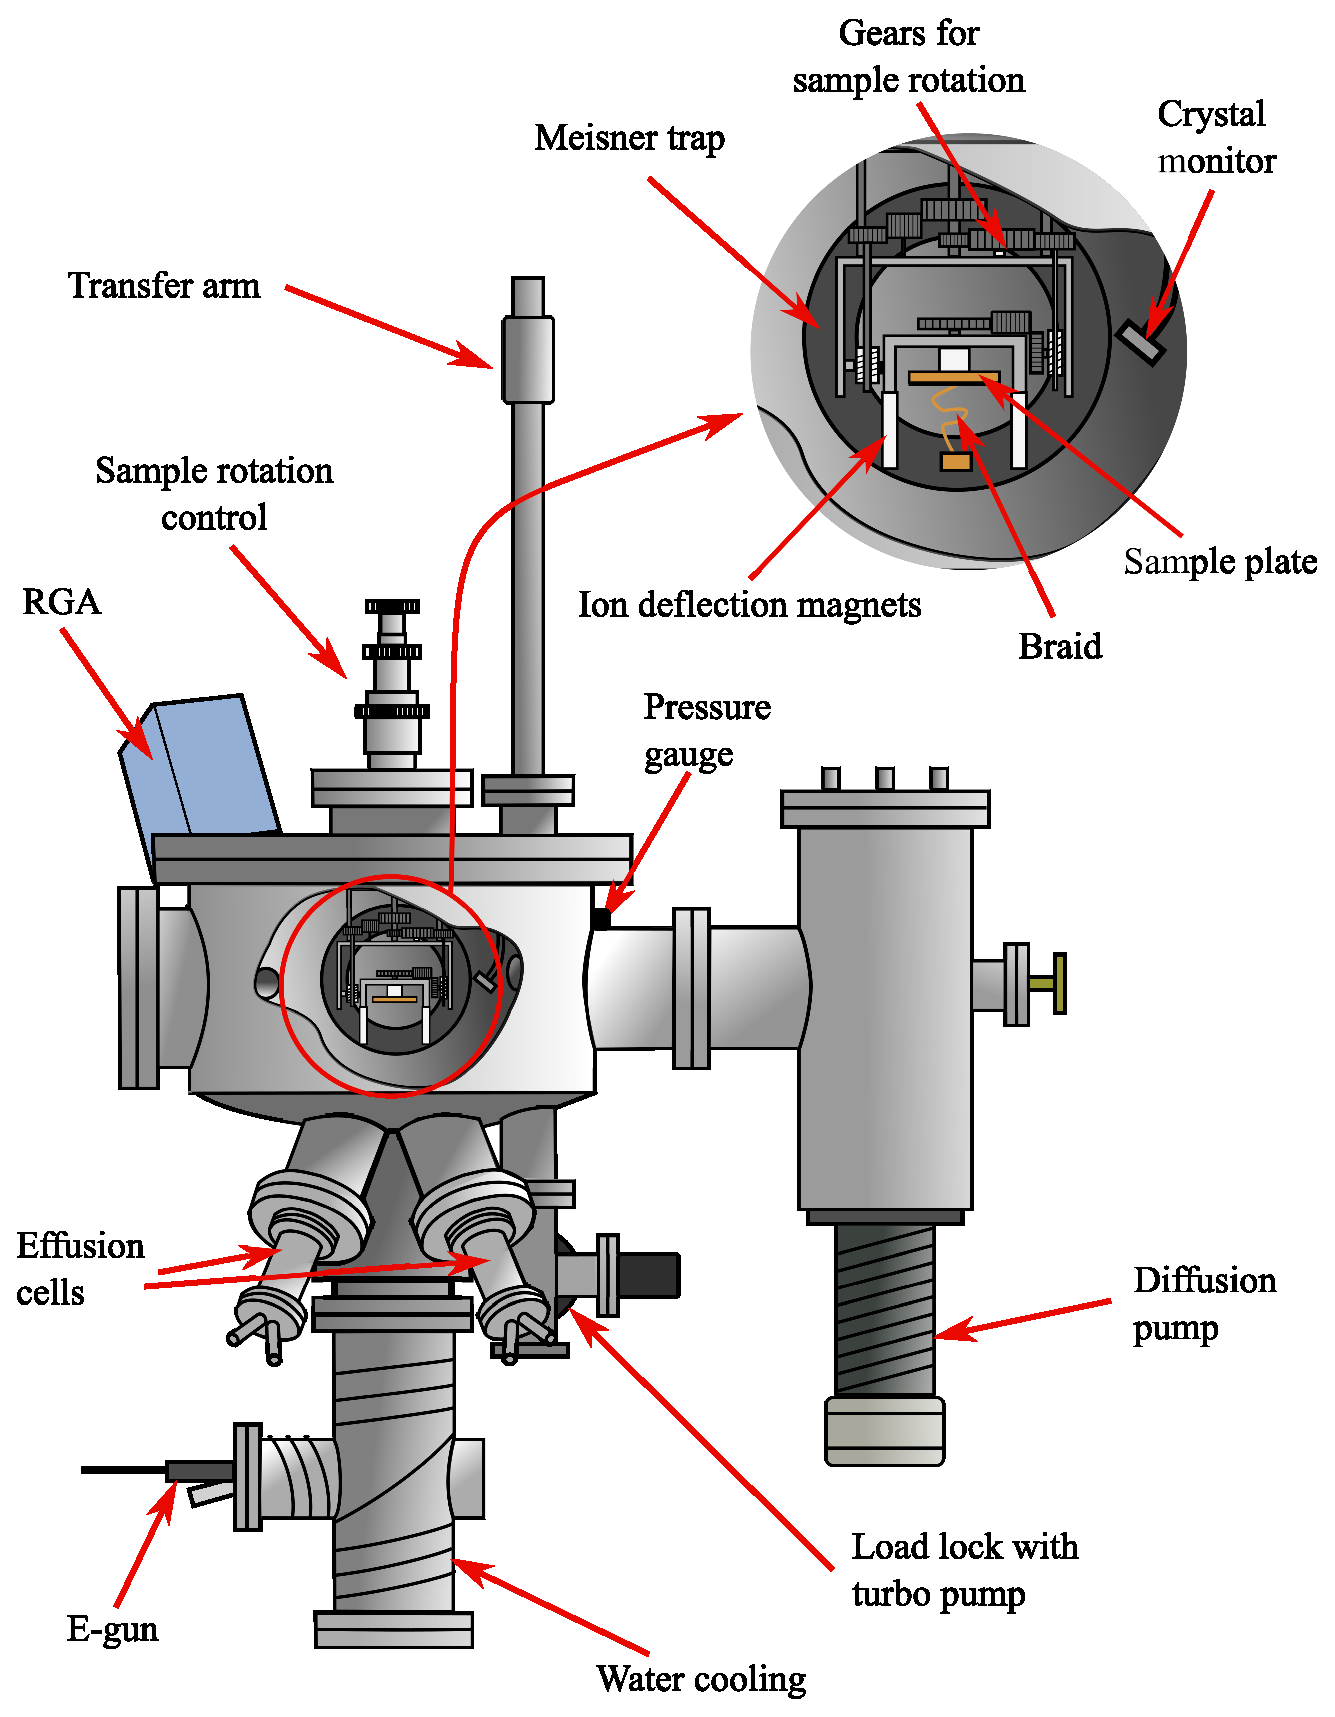
\includegraphics[width=0.5\linewidth]{slimshady_new}
	\caption{An example of how to place a figure with a caption and a lebel that you can use to cross reference the figure. Don't forget to cist the source of copied figures \cite{Batley2015} and put the label after the caption to make the cross referenced figure number correct.}
	\label{fig:fig_label}
\end{figure}

Always make sure that every figure is referred to in the text. Here, for example, figure \ref{fig:fig_label} shows one of our instruments. Tables work just like figurwes - see table \ref{tab:table_ex} for example

Non quam lacus suspendisse faucibus interdum posuere lorem ipsum dolor. Eu nisl nunc mi ipsum faucibus. Justo eget magna fermentum iaculis eu. Lacus suspendisse faucibus interdum posuere lorem. Fusce ut placerat orci nulla pellentesque dignissim enim. Vitae proin sagittis nisl rhoncus mattis rhoncus. Commodo nulla facilisi nullam vehicula ipsum. Nunc sed velit dignissim sodales ut eu. Elit pellentesque habitant morbi tristique senectus et netus et malesuada. Enim sit amet venenatis urna cursus. Phasellus vestibulum lorem sed risus ultricies. Magna eget est lorem ipsum dolor. Nulla aliquet porttitor lacus luctus accumsan. Vitae et leo duis ut. Nec tincidunt praesent semper feugiat nibh sed pulvinar proin gravida. Phasellus faucibus scelerisque eleifend donec pretium vulputate sapien nec. Amet risus nullam eget felis eget. Sodales ut etiam sit amet. Nisl condimentum id venenatis a. Neque viverra justo nec ultrices dui.

Vitae aliquet nec ullamcorper sit amet risus nullam eget felis. Egestas egestas fringilla phasellus faucibus scelerisque eleifend donec pretium. In est ante in nibh mauris cursus. Cursus in hac habitasse platea dictumst quisque sagittis. Orci ac auctor augue mauris augue neque gravida. Nullam ac tortor vitae purus faucibus ornare suspendisse. Diam donec adipiscing tristique risus nec feugiat in. Leo vel fringilla est ullamcorper eget nulla facilisi etiam. Eu augue ut lectus arcu bibendum at. In fermentum posuere urna nec tincidunt praesent. Ornare quam viverra orci sagittis eu volutpat odio. Pellentesque habitant morbi tristique senectus et.

\begin{table}
	\begin{center}
\begin{tabular}{ |p{3cm}||p{3cm}|p{3cm}|p{3cm}|  }
	\hline
	\multicolumn{4}{|c|}{Country List} \\
	\hline
	Country Name     or Area Name& ISO ALPHA 2 Code &ISO ALPHA 3 Code&ISO numeric Code\\
	\hline
	Afghanistan   & AF    &AFG&   004\\
	Aland Islands&   AX  & ALA   &248\\
	Albania &AL & ALB&  008\\
	Algeria    &DZ & DZA&  012\\
	American Samoa&   AS  & ASM&016\\
	Andorra& AD  & AND   &020\\
	Angola& AO  & AGO&024\\
	\hline
\end{tabular}
\caption{Tables are always a git of a pain in \LaTeXe - but here is an example table taken from \url{https://www.overleaf.com/}. Make sure the label goes after the caption for figures and tables!}
\label{tab:table_ex}
\end{center}	
\end{table}

Lorem ipsum dolor sit amet. Ipsum dolor sit amet consectetur adipiscing elit. Tortor vitae purus faucibus ornare suspendisse sed nisi lacus. Quis enim lobortis scelerisque fermentum dui faucibus in ornare quam. Turpis egestas sed tempus urna. Id nibh tortor id aliquet. Sed tempus urna et pharetra pharetra massa. Sit amet mauris commodo quis imperdiet. Sed felis eget velit aliquet sagittis id. Id diam maecenas ultricies mi eget mauris. Aliquet nec ullamcorper sit amet risus nullam eget felis. Nascetur ridiculus mus mauris vitae. Ultrices vitae auctor eu augue ut lectus. Dolor sed viverra ipsum nunc aliquet. Consequat ac felis donec et odio pellentesque diam volutpat commodo. Fermentum dui faucibus in ornare. Blandit massa enim nec dui nunc mattis. Dictum varius duis at consectetur lorem donec massa sapien. Sed arcu non odio euismod lacinia at quis.

Aliquam vestibulum morbi blandit cursus risus at ultrices. Euismod nisi porta lorem mollis aliquam ut. Pellentesque nec nam aliquam sem et tortor. Nunc sed augue lacus viverra vitae congue eu consequat ac. Feugiat nisl pretium fusce id velit ut. Dolor magna eget est lorem ipsum dolor sit. Faucibus ornare suspendisse sed nisi lacus sed viverra tellus. In nulla posuere sollicitudin aliquam. Habitant morbi tristique senectus et netus et malesuada. Tempor id eu nisl nunc mi ipsum faucibus vitae. Posuere morbi leo urna molestie at elementum. Euismod quis viverra nibh cras pulvinar mattis. Egestas pretium aenean pharetra magna ac placerat. Sit amet volutpat consequat mauris nunc congue nisi vitae suscipit. Vel pharetra vel turpis nunc eget lorem dolor. Id consectetur purus ut faucibus pulvinar elementum.

Volutpat maecenas volutpat blandit aliquam etiam. Magna fringilla urna porttitor rhoncus dolor purus non enim praesent. Ornare quam viverra orci sagittis. Consequat id porta nibh venenatis cras sed felis eget velit. Amet consectetur adipiscing elit ut aliquam purus sit. Ultrices tincidunt arcu non sodales neque. Vitae congue mauris rhoncus aenean vel elit scelerisque. Nunc faucibus a pellentesque sit amet porttitor. Faucibus vitae aliquet nec ullamcorper sit amet risus. Fringilla urna porttitor rhoncus dolor purus non enim praesent. Diam maecenas ultricies mi eget mauris. Amet aliquam id diam maecenas ultricies. Massa enim nec dui nunc. Tempor nec feugiat nisl pretium fusce. Risus nullam eget felis eget nunc. Sed odio morbi quis commodo odio. Porttitor massa id neque aliquam vestibulum morbi blandit cursus. Vitae tempus quam pellentesque nec nam aliquam sem.

At ultrices mi tempus imperdiet nulla malesuada. Cum sociis natoque penatibus et magnis. Mattis pellentesque id nibh tortor id aliquet lectus proin nibh. Facilisis volutpat est velit egestas dui id ornare arcu. Cras ornare arcu dui vivamus arcu felis bibendum. Senectus et netus et malesuada. Nunc mattis enim ut tellus. Eu mi bibendum neque egestas congue quisque egestas diam in. Mattis nunc sed blandit libero. A cras semper auctor neque vitae tempus. Porttitor eget dolor morbi non arcu. Magna ac placerat vestibulum lectus mauris ultrices. Vulputate sapien nec sagittis aliquam malesuada bibendum. %% file path for chapter tex files 
\include{Chapters/Chapter_2/Chapter_2_File}
%\include{Chapters/Chapter_3/Chapter_3_File}
%\include{Chapters/Chapter_4/Chapter_4_File}
%\include{Chapters/Chapter_5/Chapter_5_File}
%\include{Chapters/Chapter_6/Chapter_6_File}


%\appendix
\chapter{Material not in a chapter}
This is the first appendix.

\section{Bits of \LaTeX advice}

\begin{enumerate}
	\item Do look at the output log and try to understand any errors - they are sometimes important!
	\item In the final pdf, do a search for ? - it is what \LaTeX will give when a reference is missing. Having missing references in your submitted thesis is, at best, embarrassing and potentially a failing matter.
	\item A good quality bib file is important - make sure that entries are consistent in whether journals are abreviated, capitalised and how Author names are presented. A good way to do this is to use Mendeley to import your bib file and then use its doi lookup feature which will re-write your bibliogrpahy entries in a standardised form. You then export the bibliography back oit as a bib file.
	\item Be particularly careful about older papers where the doi may not be easy to track down. Also watch out for JETP Letters that you are being consistent in citing the English language version (or the Russian, but don't mix and match!)
	\item Although \LaTeX guides may show you how to assemble a multi-part fgure from within \LaTeX, it can be hard to make sub-plots appear exactly the same size. We recommend using something like Inkscape to assemble the parts of a figure and lay them out nicely. Be careful if saving to pdf files thatr the fonts are preserved - otherwise you can lose greek symbols.
	\item If preparing figures in Origin, set the plot size to be exactly the right size or exactly double size and then scale fonts and symbols accordingly. Use Origin's ability to copy formatting between graphs to make everything nicely consistent (e.g. frame sizes, thicknesses, coolour schemes, point sizes and shapes).
	\item In general resist the temptation to put [H] when placing figures and tables - in most cases it is better to let \LaTeX work out where to put things. It can get tricky if you have a lot of figures one after another (perhaps a single multi-part figure is what you need?) - the placement option [p] can alos help to move floats to a separate page of figures. See also the \textit{afterpage} package. 
\end{enumerate}
%\include{Appendix2/Appendix2}
%. More appendicies here.
\addcontentsline{toc}{chapter}{References} % Adds References to contents page
\bibliographystyle{ieeetr_me} % bibliography style
\renewcommand{\bibname}{References} 
\bibliography{References/library} % References file
\end{document}